\documentclass[letterpaper, reqno,11pt]{article}
\usepackage[margin=1.0in]{geometry}
\usepackage{color,latexsym,amsmath,amssymb,graphicx,float,listings,tikz}
\usepackage{hyperref}

\hypersetup{
colorlinks=true,
linkcolor=magenta,
filecolor=magenta,
urlcolor=cyan,
}

\lstset{
basicstyle=\ttfamily,
columns=fullflexible,
frame=single,
breaklines=true,
postbreak=\mbox{\textcolor{red}{$\hookrightarrow$}\space},
}

\graphicspath{ {images/} }

\begin{document}
\pagenumbering{arabic}
\title{PHYS 403 Homework 7}
\date{14/04/24}
\author{Xander Naumenko}
\maketitle

{\medskip\noindent\bf Question I1.} To calculate the partition function we can sum over possible states:
\[
Z=\sum_{s_1\in \{-1,1\}}\cdots \sum_{s_N\in \{-1,1\}}e^{\beta Js_1s_2}\cdots e^{\beta Js_{N-1}s_N}
.\]

Note that for general $2\times 2$ matrices $A,B$ and $i,k\in \{1,2\}$, it's true that $\sum_{j\in \{1,2\}}A_{ij}B_{jk}=(AB)_{ik}$. In particular we have $\sum_{s_2\in \{-1,1\}}M_{s_1s_2}M_{s_2s_3}=\left( M^2 \right)_{s_1s_3}$, where $M$ here and later is being indexed with $1$ for it's first entry and $-1$ for the second. Since $M_{ij}=e^{\beta Jij}$ appears in the sum, we can repeatedly apply this identity to get
\[
Z=\sum_{s_1\in \{-1,1\}}(M^{N})_{s_1s_1}=\text{tr} M^{N}
.\]

{\medskip\noindent\bf Question I2.} This is just some computation with linear algebra:
\[
    \begin{vmatrix} e^{\beta J}-\lambda&e^{-\beta J}\\e^{-\beta J}&e^{\beta J}-\lambda \end{vmatrix} =0\implies \lambda^2-2e^{\beta J}\lambda+\left( e^{2\beta J}-e^{-2\beta J} \right)=0
\]
\[
\implies \lambda_{\pm} = e^{\beta J}\pm e^{-\beta J}
.\]
For the eigenvectors the system is easy enough to just guess and check the correct vectors:
\[
M \vec v_{\pm}=\lambda_{\pm} \vec v_{\pm}\implies \vec v_{\pm}= \frac{1}{\sqrt{2}}\begin{pmatrix} 1\\ \pm 1 \end{pmatrix} 
.\]

{\medskip\noindent\bf Question I3.} Since all the $i$s are symmetric (since we're using periodic boundary conditions), the expression is unchanged if we assume that $i=1$. Then we have
\[
    \langle s_{i+x}s_i \rangle =\langle s_{x+1}s_1 \rangle =\frac{1}{Z}\sum_{s} s_1 s_{x+1}e^{-\beta H(s)}=\frac{1}{Z}\sum_{s} s_1 s_{x+1}e^{\beta Js_1s_2}\cdots e^{\beta Js_{N-1}s_N}
.\]
Using the same trick as in part 1, for $i\neq 1, i\neq x+1$, we can use the fact that $M_{ij}=e^{\beta J ij}$ to get
\[
    \langle s_{i+x}s_i \rangle= \frac{1}{Z}\sum_{s_1\in \{-1,1\}}\sum_{s_{x+1}\in \{-1,1\}}s_1s_{x+1}(M^{x})_{s_1s_{x+1}}(M^{N-x})_{s_{x+1}s_1}
.\]
To simplify this, note that $s_i=\left( \sigma^{z} \right)_{s_is_i}$, and since the matrix combination argument from part 1 doesn't rely on the specific form of $M$, it applies to $\sigma^{z}$ as well:
\[
    \langle s_{i+x}s_i \rangle= \frac{1}{Z}\sum_{s_1\in \{-1,1\}}\left( \sigma^{z}M^{x}\sigma^{z}M^{N-x} \right)_{s_is_i}=\frac{1}{Z}\text{tr}\left[ \sigma^{z}M^{x}\sigma^{z}M^{N-x} \right]
\]
\[
=\frac{1}{Z}\text{tr}\left[ \left(\sigma^{z}M^{x}\sigma^{z}M^{N-x}\right)^{T} \right]=\frac{1}{Z}\text{tr}\left[ M^{N-x}\sigma^{z}M^{x}\sigma^{z} \right]
.\]
The last step uses the fact that all the matrices in question are symmetric. To evaluate it, as the hint suggests we work in the eigen basis of $M$. From the result of part 2, we have that $\sigma^{z}\vec v_+=v_-, \sigma^{z}\vec v_-=v_+$. Computing the trace:
\[
\frac{1}{Z}\text{tr}\left[ M^{N-x}\sigma^{z}M^{x}\sigma^{z} \right]=\frac{1}{Z}\left( \vec v_+^{T}(M^{N-x}\sigma^{z}M^{x}\sigma^{z})\vec v_++\vec v_-^{T}(M^{N-x}\sigma^{z}M^{x}\sigma^{z})\vec v_- \right)
\]
\[
 =\frac{1}{Z}\left( \lambda_-^{N-x}\lambda_+^{x}+\lambda_-^{x}\lambda_+^{N-x} \right)
.\]
We can compute $Z$ using the same method:
\[
Z=\vec v_+^{T}M^{N}\vec v_+ + \vec v_-^{T}M^{N}\vec v_- = \lambda_+^{N}+\lambda_-^{N}
.\]
Putting it together we get
\[
\langle s_{i+x}s_i \rangle = \frac{1}{\lambda_-^{N}+\lambda_+^{N}} \left( \lambda_-^{N-x}\lambda_+^{x}+\lambda_-^{x}\lambda_+^{N-x} \right)
\]
where $\lambda_+$ and $\lambda_-$ are defined as in part 2.

{\medskip\noindent\bf Question I4.} In the limit of $N\to\infty$, we have that $Z=\lambda_-^{N}+\lambda_+^{N}\to \lambda_+^{N}\left( 1+\left(\frac{\lambda_-}{\lambda_+}\right)^{N} \right) \to\lambda_+^{N}$ and
\[
\langle s_{i+x}s_i \rangle = \frac{\lambda_+^{N-x}}{Z}\left( \left(\frac{\lambda_-}{\lambda_+}\right)^{N-x}\lambda_+^{x}+\lambda_-^{x} \right) =\frac{\lambda_+^{N-x}\lambda_-^{x}}{\lambda_+^{N}}=\left( \frac{\lambda_+}{\lambda_-} \right) ^{-x}=e^{-x\log \frac{\lambda_+}{\lambda_-}}
.\]
From this expression we see that $\xi=\left(\log \frac{e^{\beta J}+e^{-\beta J}}{e^{\beta J}-e^{-\beta J}}\right)^{-1}=\left(\log \frac{e^{2\beta J}+1}{e^{2\beta J}-1}\right)^{-1}$. In the low temperature limit, we asymptotically get
\[
\xi = \left(\log \frac{e^{2\beta J}+1}{e^{2\beta J}-1}\right)^{-1}\to \frac{1}{2}e^{\frac{2J}{k_BT}}\to\infty
.\]
Interestingly $\xi$ is a finite number for all positive temperatures, so there is no critical temperature at which the magnet spontaneously organizes itself.

{\medskip\noindent\bf Question I5.} From the partition function in the low temperature limit:
\[
\langle E \rangle =- \frac{\partial}{\partial\beta}\log Z=-N\frac{\partial}{\partial\beta}\log\left( e^{\beta J}+e^{-\beta J} \right)=-N \frac{Je^{\beta J}-Je^{-\beta J}}{e^{\beta J}+e^{-\beta J}}
\]
\[
\implies \frac{\Delta E}{N}= -J\left(\frac{e^{2\beta J}-1}{e^{2\beta J}+1}-1\right)= \frac{2J}{e^{2\beta J}+1}
.\]
Each domain wall has energy $J$ (since it involves one spin flip), so the density is just $n_{DW}= \frac{2}{e^{2\beta J}+1}$. Since we're in 1 dimension the length is just the inverse of density, so $l_{DW}=\frac{1}{2}\left( e^{2\beta J}+1 \right) $. This is almost the same form we found for $\xi$ above, just with an offset of $\frac{1}{2}$. The physical reason that these are related is that the distance between domain walls is, almost by definition, the distance at which the spin is expected to flip. Once the distance is far enough for that the spins start flipping the correlation between those spins will decrease, so effectively $l_{DW}$ and $\xi$ measure the same thing.

\newpage

{\medskip\noindent\bf Question II1.} There are two symmetries of the model: reflection and rotation. More precisely, replacing $\vec S_i\to -\vec S_i$ is reflection symmetry, while multiplying $\vec S_i$ by a rotation matrix is rotation symmetry.

{\medskip\noindent\bf Question II2.} Any state that has every spin nonzero and aligned in the same direction is a ground state, since in this case every $\vec S_i\cdot\vec S_j=1\forall i,j$ which obviously minimizes the energy. Since any direction of spin is valid, it is a continuum with infinitely many ground states. At $T=0$ reflection symmetry of $\vec S_i\to \vec S_j$ is broken.

{\medskip\noindent\bf Question II3.} Let $\vec m$ be the mean field. From the rotation symmetry, assume that $\vec m$ points along the $z$ axis. Then we have
\[
H=-J\sum_{i,j}\left( \vec m+\delta s_i \right) \left( \vec m+\delta s_j \right) =\frac{J}{2}qN\vec m^2-qJ\vec m\cdot \left( \sum_{i}\vec S_i \right) 
.\]
Here $q$ is the number of neighbors, given we're in a cubic lattice this is 6 but I'll leave it as a general parameter. Let $E_0=\frac{J}{2}qN\vec m^2$

{\medskip\noindent\bf Question II4.} 
\[
Z=\sum_{\vec m}e^{-\beta F(m)}
\]
\[
e^{-\beta F(\vec m)}=e^{-\beta E_0}\sum_{\{S_i\}}e^{-\beta\left(Jq\vec m\cdot \sum_{i}\vec S_i \right) }=e^{-\beta E_0}\left( \sum_{s\in \{-1, 0, 1\}}e^{\beta Jqs|m|} \right) 
\]
\[
\implies F(\vec m)=-E_0+\frac{N}{\beta}\log \left( 2\cosh\left( \beta Jq|\vec m| \right) +1 \right) 
.\]

{\medskip\noindent\bf Question II5.} Let $m=|\vec m|$. Self consistency is equivalent to free energy minimization:
\[
    \frac{dF}{dm}=2E_0-N \frac{2 \sinh\left( \beta Jqm \right) }{2\cosh \left( \beta Jqm \right) +1}=0
\]
\[
\implies m= \frac{2\sinh\left( \beta Jqm \right)}{2\cosh \left( \beta Jqm \right) +1}
.\]

{\medskip\noindent\bf Question II6.} The critical temperature occurs when the system goes from having multiple local minima in the free energy to just one. Graphically this occurs when the slope of the expression from the previous part is 1 at most, and since it is steepest at $m=0$, we can expander there
\[
    \left( \frac{2\sinh\left( \beta Jqm \right)}{2\cosh \left( \beta Jqm \right) +1} \right)'= \frac{\beta Jq 2\cosh\left( \beta J qm \right) \left( 2\cosh\left( \beta J qm \right) +1 \right) -4\beta Jqm\sinh^2\left( \beta Jqm \right) }{\left( 2\cosh\left( \beta Jqm \right) +1 \right) ^2}
.\]
Applying $m=0$ and setting it equal to 1 gives
\[
\frac{2\beta Jq}{3}=1\implies T=\frac{2Jq}{3k_B}
.\]

{\medskip\noindent\bf Question II7.} The requirements here are mostly the same as the Ising model case. The free energy must be analytic and lower bounded, and reflection symmetry means that only even powers are allowed. Rotational symmetry means that there's no direction dependence meaning only terms with $|\vec m|$ in them, so the form will be $f(\vec m)\approx a|\vec m|^2+b|\vec m|^4$.

\newpage

{\medskip\noindent\bf Question III.} Minimizing:
\[
\frac{df}{dx}=2a\phi+4b\phi^3+6c\phi^5=0\implies \phi= \pm\sqrt{\frac{1}{3c}\left( -b\pm \sqrt{b^2-3ac} \right)} \text{ or }\phi=0
.\]
This gives five possible roots. Since $f$ is even just consider $\phi\geq 0$, by symmetry the others are equivalent. Since these equations involve nested radicals, I'll use Mathematica for symbolic solving (given the hint I realize there might be some nice simplifications, but I'm lazy). Denote $\phi_\pm(a)=\sqrt{\frac{1}{3c}\left( -b\pm \sqrt{b^2-3ac} \right)}$. 

Any discontinuity in $\phi$ will occur when $f(\phi_\pm(a))=0$, since that's the point that $\phi_+$ or $\phi_-$ switch from being global minimum to $\phi=0$ being the global minimum (if they are even minima at all to begin with, which we'll check after). Symbolically solving the equation $f(\phi_\pm(a))=0$ for $b<0,c<0$ we get that $a=\frac{b^2}{4c}$ for $\phi_+$ and $a=0$ for $\phi_-$. Symbolically computing, we also find that $f''\left(\phi_+\left(\frac{b^2}{4c}\right)\right)=\frac{2b^2}{3c}>0$ and $f''\left( \phi_-\left( 0 \right)  \right) = \frac{-2b^2}{3c}<0$.

Since we only care about minimums in the free energy we can discard $\phi_-$ since we just found it to be a maximum (at least when it crosses the $f(\phi)=0$ line where we care about it, and so there will be only one discontinuity in $\phi$ at $a=\frac{b^2}{4c}$. As the question asks, this discontinuity does not occur at $a=0$ as it did for the $b>0$ case we investigated in class.

Next we need to check that $f'(a)$ (note that here $f$ is a function of $a$ not $\phi$, from context it should be clear which one I mean) is discontinuous at $a=\frac{b^2}{4c}$. To be explicit, summarizing the above paragraphs gives
\[
f(a)=\begin{cases}
    \frac{a}{3c}\left( -b\pm \sqrt{b^2-3ac}\right)+b\left( \frac{1}{3c}\left( -b\pm \sqrt{b^2-3ac} \right)\right)^2+c\left( \frac{1}{3c}\left( -b\pm \sqrt{b^2-3ac} \right)\right)^3 &\text{ if }a\leq \frac{b^2}{4c}\\
    0&\text{ else}
\end{cases}
.\]
Symbolically the first case of the above expression was computed and evaluated at $a=\frac{b^2}{4c}$ to give $\lim_{a\to \frac{b^2}{4c}^{-}}f'(a)=-\frac{b}{2c}$. Clearly we have $\lim_{a\to \frac{b^2}{4c}^{+}}f'(a)=\lim_{a\to \frac{b^2}{4c}^{+}}0=0$, so this gives that $\frac{d}{da}f(a)$ is not continuous and thus $a=\frac{b^2}{4c}$ is a first order phase transition.

For what it's worth graphs of the phase two cases in the expression for $f(a)$ above can be seen in figure \ref{fig:III}. All of the above proof holds independently of the graph, but what's going on there is much more intuitive than just stating results from a symbolic solver.

\begin{figure}[htpb]
    \centering
    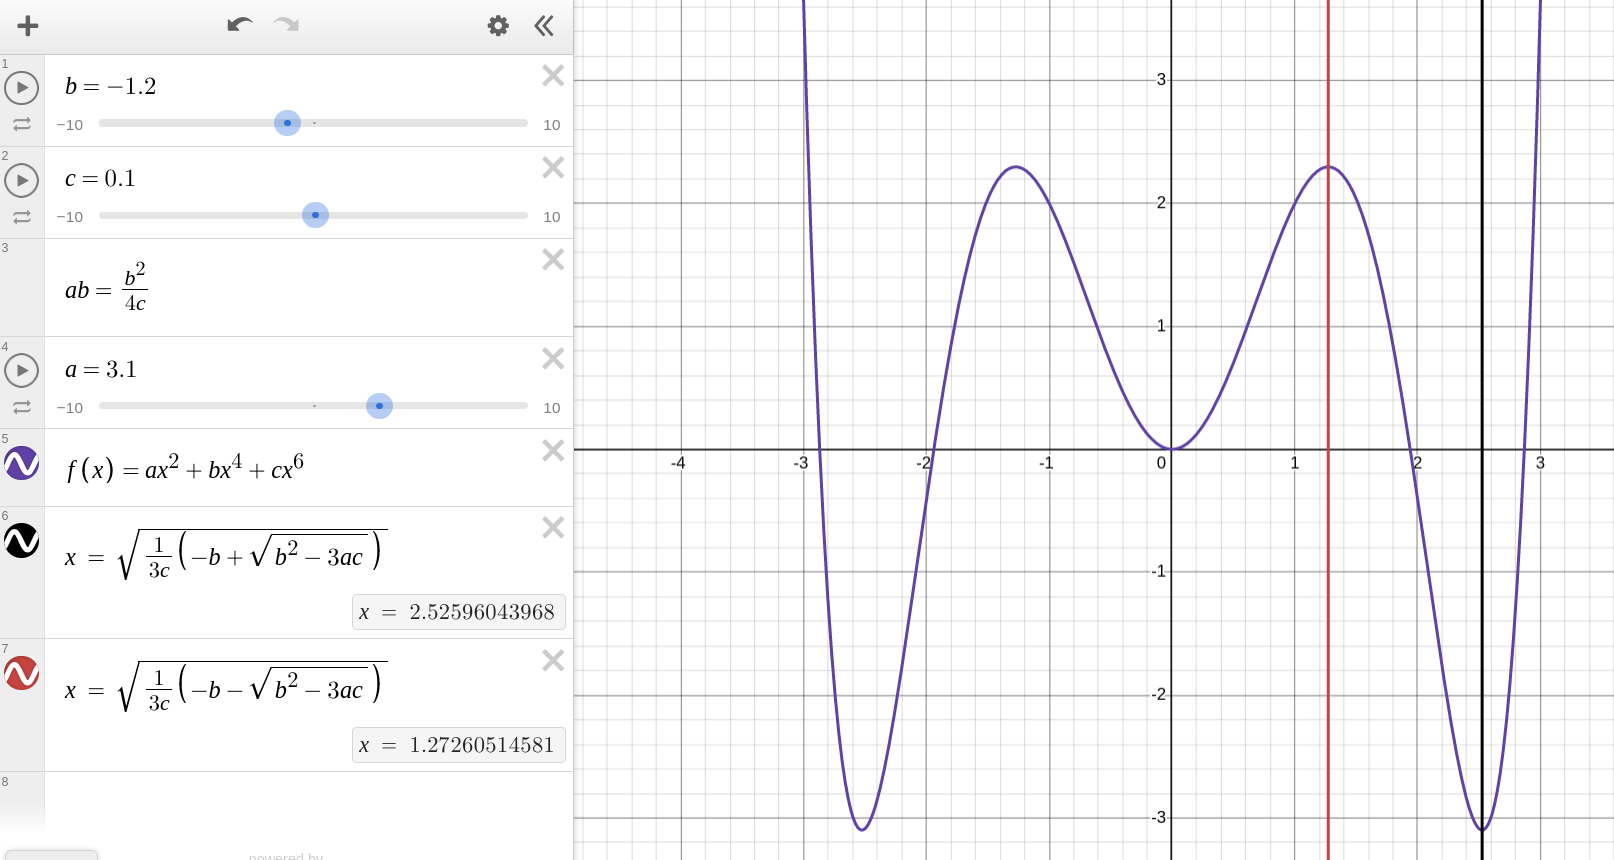
\includegraphics[width=0.8\textwidth]{asmall}
    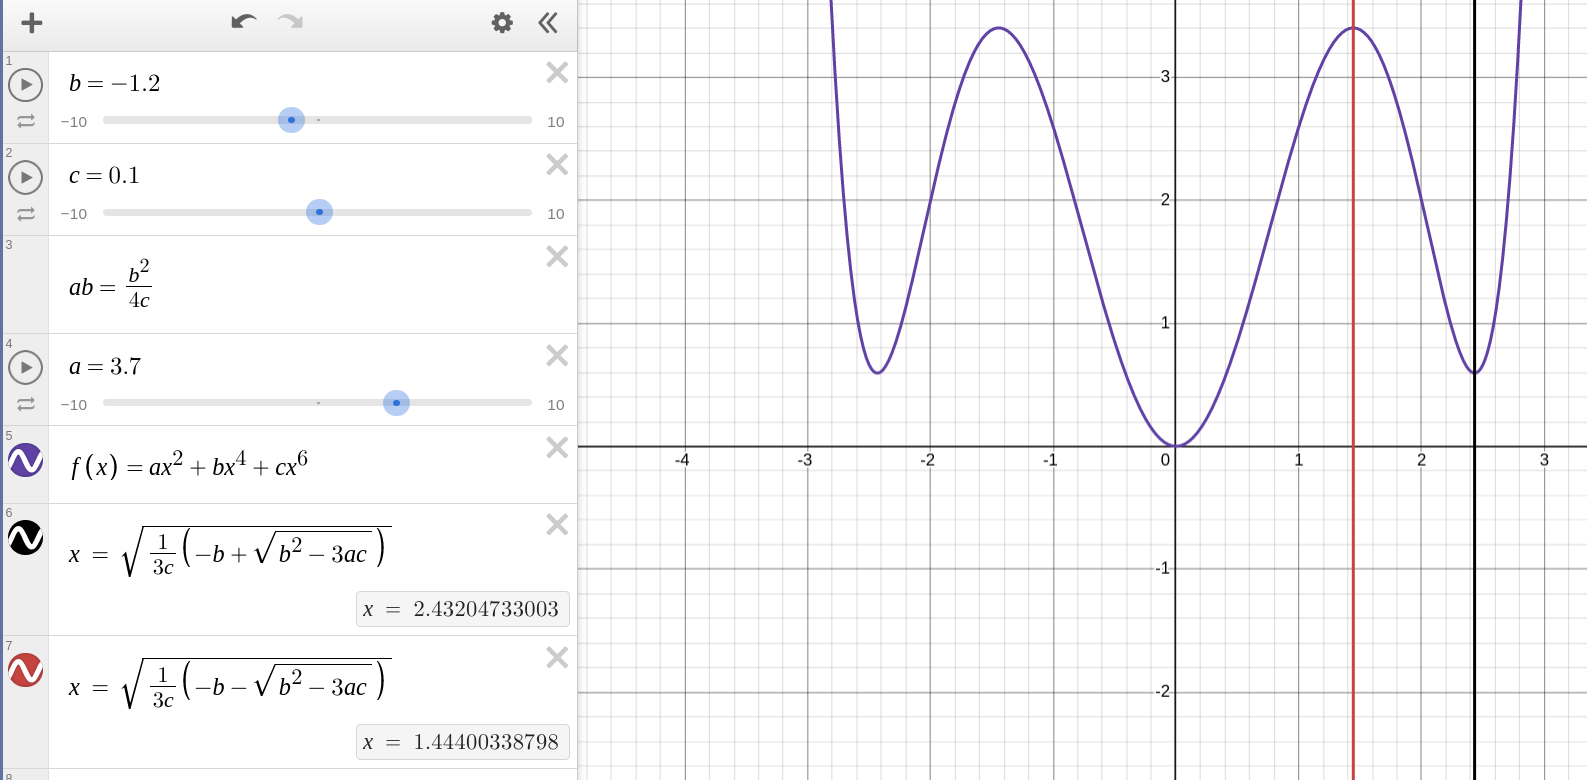
\includegraphics[width=0.8\textwidth]{abig}
    \caption{Quick Desmos graph of $f(a)$ for $a<\frac{b^2}{4c}$ (top) vs $a>\frac{b^2}{4c}$ (bottom). Again, this isn't required for the proof I gave but it's a good guide for intuition.}
    \label{fig:III}
\end{figure}



\end{document}
